%%「論文」,「レター」,「レター(C分冊)」,「技術研究報告」などのテンプレート
%% v3.4 [2023/09/12]
%% 1. 「論文」
\documentclass[paper]{ieicej}
% \documentclass[technicalreport]{ieicej}

% \documentclass[invited]{ieicej}% 招待論文
%\documentclass[survey]{ieicej}% サーベイ論文
%\documentclass[comment]{ieicej}% 解説論文
\usepackage[dvipdfmx]{graphicx,xcolor}
%%\usepackage[dvips]{graphicx}
\usepackage[fleqn]{amsmath}
%\usepackage{amsthm}
\usepackage{newtxtext}% 英数字フォントの設定を変更しないでください
\usepackage[varg]{newtxmath}% % 英数字フォントの設定を変更しないでください
%\usepackage{amssymb}
%\usepackage{bm}
\usepackage{listings,jvlisting} %日本語のコメントアウトをする場合jvlisting(もしくはjlisting)が必要
%ここからソースコードの表示に関する設定
\lstset{
  basicstyle={\ttfamily},
  identifierstyle={\small},
  commentstyle={\smallitshape},
  keywordstyle={\small\bfseries},
  ndkeywordstyle={\small},
  stringstyle={\small\ttfamily},
  frame={tb},
  breaklines=true,
  columns=[l]{fullflexible},
  numbers=left,
  xrightmargin=0zw,
  xleftmargin=3zw,
  numberstyle={\scriptsize},
  stepnumber=1,
  numbersep=1zw,
  lineskip=-0.5ex,
  % extendedchars=false, % ★ 日本語の縦書き化を防止
}
\renewcommand{\lstlistingname}{プログラム}% ソースコードのキャプションの名称

\setcounter{page}{1}

\field{A}
\jtitle{状態遷移図ベースのコード生成とログ可視化機能を備えたセンサネットワーク実機検証基盤の開発}
\etitle{}
\authorlist{%
 \authorentry[24w6047a@shinshu-u.ac.jp]{辻村篤志}{Atsushi Tsujimura}{信州大学}\MembershipNumber{}
 \authorentry{小林侑生}{Yu Kobayashi}{信州大学}\MembershipNumber{}
 \authorentry{不破泰}{Yasushi Fuwa}{信州大学}\MembershipNumber{}
 \authorentry{アサノデービッド}{David Asano}{信州大学}\MembershipNumber{}
 %\authorentry{和文著者名}{英文著者名}{所属ラベル}\MembershipNumber{}
 %\authorentry[メールアドレス]{和文著者名}{英文著者名}{所属ラベル}\MembershipNumber{}
 %\authorentry{和文著者名}{英文著者名}{所属ラベル}[現在の所属ラベル]\MembershipNumber{}
}
\affiliate[Nagano]{信州大学 〒380-0928 長野県長野市若里4-17-1}
 {Shinshu University, 4--17--1 Wakasato, Nagano-shi, 
  Nagano 380--8553 Japan}
%\affiliate[所属ラベル]{和文所属}{英文所属}
%\paffiliate\[]{}
%\paffiliate[現在の所属ラベル]{和文所属}
\jalcdoi{???????????}% ← このままにしておいてください

\begin{document}
\begin{abstract}
%和文あらまし 500字以内
センサネットワークの開発は幅広い専門知識と多大な工数を要する。先行研究では、センサネットワークの動作を表す状態遷移図からコードを生成し、汎用ハード上で動作する環境が構築されてきた。本研究ではその環境を拡張し、その上で実用的な無線通信プロトコルを実装・検証した。その過程で汎用ハード上でのプロトコルの動作が確認しづらいことを課題として認識し、デバッグ用ログ出力とそれを可視化・ステップ実行できる環境を開発しデバッグ効率の向上を図った。
\end{abstract}
\begin{keyword}
%和文キーワード 4〜5語
無線センサーネットワーク、無線通信プロトコル、状態遷移図、コード生成、ログ可視化
\end{keyword}

\begin{eabstract}
%英文アブストラクト 100 words
The development of sensor networks requires extensive expertise and significant effort. Previous research has generated code from state transition diagrams representing the behavior of sensor networks, establishing an environment that operates on general-purpose hardware. This study expands that environment and implements and verifies practical wireless communication protocols. During this process, we recognized the difficulty in confirming the operation of protocols on general-purpose hardware as a challenge and developed an environment for debugging log output and visualizing and step-executing it to improve debugging efficiency.
\end{eabstract}

\begin{ekeyword}
%英文キーワード
wireless sensor networks, wireless communication protocols, state transition diagrams, code generation, log visualization
\end{ekeyword}
\maketitle

% _/_/_/_/_/_/_/_/_/_/_/_/_/_/_/_/_/_/_ 1章 /_/_/_/_/_/_/_/_/_/_/_/_/_/_/_/_/_/_/_/_/_/_/_/_/_/_/_/_/_/_/
\section{はじめに}
\subsection{背景}
近年、無線センサネットワーク(Wireless Sensor Network:WSN)は、環境モニタリングやスマートシティ、インフラ監視、農業、ヘルスケアなど、さまざまな分野での応用が期待されている。実際、WSNを含むIoTデバイスの数は2020年時点で約130億台に達し、年率20%で増加しており、2025年には300億台弱に到達すると予測されている\cite{jst2022}. また、MDPIの報告によれば、WSNノードの数は2012年の約4.5億台から2022年には約20億台へと拡大しており\cite{mdpi2021}、その研究および実用の両面での発展が顕著である。  
しかし、これらのシステムを構築するためには、複雑な通信プロトコル設計やデータ処理アルゴリズムの実装が求められ、開発者には高度な専門知識と多大な工数が必要となる。そのため、システム開発の効率化や開発者支援を目的とした研究が進められている。
\vskip\baselineskip

\subsection{従来研究}
従来研究では、無線通信プロトコルの状態遷移図から自動生成したプログラムを汎用ハード上で動作させ、CSMAおよびTDMAベースのMACプロトコルを実機で実装・検証できる環境が構築されていた(旭ら)。このシステムにより基本的な通信プロトコルの動作検証が可能となったが、デバッグ方法はシリアルコンソールへのログ出力に依存しており、通信処理が高速に進むため逐次的な状態遷移を追跡することが難しかった。その結果、異常動作の原因を把握しづらく、開発効率や教育的利用の観点では十分でない点が課題として残されていた。

\vskip\baselineskip
\subsection{目的}
本研究の目的は、従来研究で課題となっていたデバッグ効率の低さを改善し、実機でのプロトコル検証をより効果的に行える環境を実現することである。そのために、状態遷移図から生成したコードの動作をログとして出力し、それを可視化・ステップ実行できる仕組みを開発した。これにより、プロトコルの動作を逐次的に把握でき、異常動作の原因究明を容易にするとともに、教育や応用実証に適した支援環境を提供することを目指す。
\vskip\baselineskip




% _/_/_/_/_/_/_/_/_/_/_/_/_/_/_/_/_/_/_ 2章 /_/_/_/_/_/_/_/_/_/_/_/_/_/_/_/_/_/_/_/_/_/_/_/_/_/_/_/_/_/_/
\section{提案システム}
\subsection{システム構成}
本研究で開発したシステムの全体構成を図\ref{fig:system-composition}に示す。本システムは、状態遷移図を入力としてC++プログラムを自動生成し、PlatformIO上でビルドを行い、汎用ハードウェア上で実行することでセンサネットワークのプロトコルの動作検証を可能とする。さらに、通信動作の状態遷移や変数値の過程をログとして記録し、ブラウザ上で状態遷移の可視化およびステップ実行を行える環境を備えている。これにより、プロトコル設計から実機検証、デバッグまでを一貫して支援することが可能となる。
\vskip\baselineskip
\begin{figure}[tb]
  \centering
  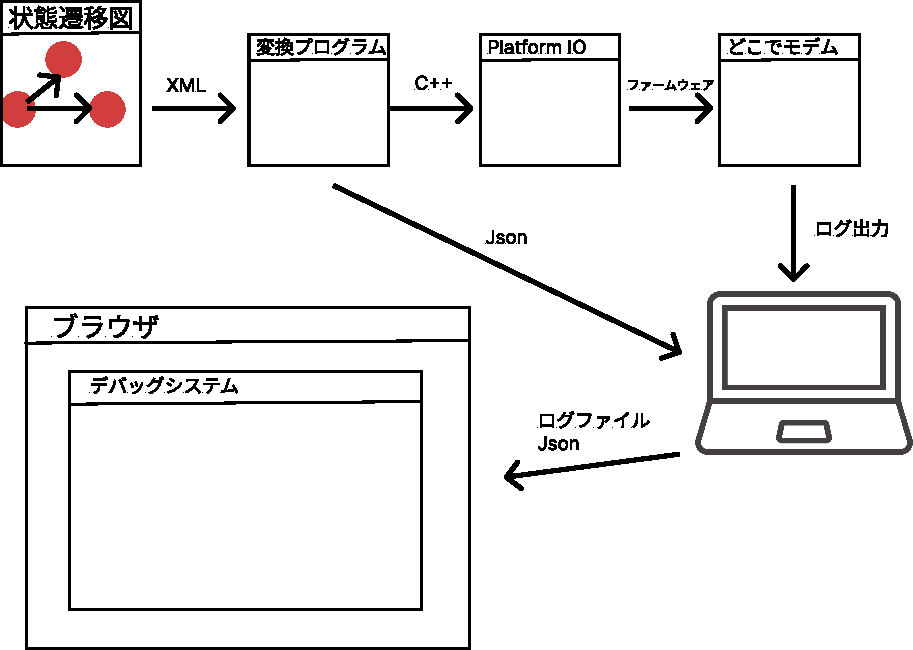
\includegraphics[width=80mm]{./images/system-composition.pdf}
  \caption{提案システムの全体構成}
  \ecaption{Block diagram of the proposed system.}
  \label{fig:system-composition}
\end{figure}


\subsection{ファームウェア生成部}
ファームウェア生成部では,無線通信プロトコルの動作をAstah Professional上の状態遷移図として設計し,XML形式で出力する。次に,変換プログラム(Python)を用いて状態遷移図のXMLをC++プログラムへ変換し,PlatformIO環境でビルドすることでファームウェアを生成する。このファームウェアは2.3節で述べる汎用ハードウェア上で実行される。

先行研究(小林ら\cite{kobayashi2023})では,状態遷移図の各要素(通信状態・遷移・初期値設定・処理内容など)をXMLファイルから抽出し,それぞれをリスト化したうえで,通信状態間の関係を解析し,C++の`switch-case`構造に変換するアルゴリズムが実装されている。本研究におけるファームウェア生成部は,この変換処理を利用しており,状態遷移図で設計されたプロトコル仕様を汎用ハードウェア上で動作するプログラムとして自動生成するものである。

図\ref{fig:state-machine}に状態遷移図の例を,プログラム\ref{converted-code}に変換後のC++コードを示す。状態遷移図で定義された「待機(LISTEN)」「受信(RECEIVE)」「送信(TRANSMIT)」の各状態と遷移関係が,`switch-case`構造によって対応づけられており,設計段階の論理構造がソースコードとして正しく反映されていることが確認できる。

\vskip\baselineskip
\begin{figure}[tb]
  \centering
  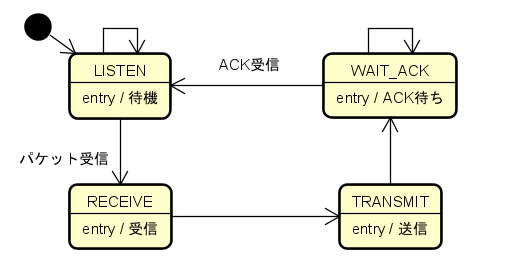
\includegraphics[width=60mm]{./images/state-machine-image.png}
  \caption{状態遷移図の例}
  \ecaption{State transition diagram.}
  \label{fig:state-machine}
\end{figure}

\begin{figure}
\begin{lstlisting}[caption={変換されたC++プログラム}, label=converted-code]
typedef enum { LISTEN, RECEIVE, TRANSMIT } NodeState;

void protocol_main() {
  switch (state) {
    case LISTEN:   updateState(RECEIVE);   break;
    case RECEIVE:  updateState(TRANSMIT);  break;
    case TRANSMIT: updateState(LISTEN);    break;
  }
}
\end{lstlisting}
\end{figure}
\vskip\baselineskip




\subsection{実行環境(ハードウェア)}
次に,実行環境について述べる。本システムでは,SAMD21マイコンを搭載した無線モデム(株式会社サーキットデザイン製どこでモデム)を用い,生成したファームウェアを書き込み実行する。このモデムは429 MHz帯で動作する汎用的な無線モデムであり,技術基準適合証明を取得しているため,実際に電波を送受信しながら通信プロトコルの検証を行うことができる。また,429 MHz帯は中山間地域において回折性能に優れており,低消費電力で長距離通信が可能なLPWA(Low Power Wide Area)通信に適している。この特性を活かすことで,将来的には登山者見守りシステムなどへの応用も期待できる。さらに,本モデムはマイコンと通信モジュールが一体化しているため,外部配線や追加ハードウェアを必要とせず,開発や実験環境の構築を容易に行うことが可能である。加えて,GPSモジュールを併用することで,位置情報の取得および1PPS信号による高精度な時刻同期を実現し,複数ノード間での無線通信プロトコルの正確な動作検証を可能としている。
\vskip\baselineskip
\begin{figure}[tb]
  \centering
  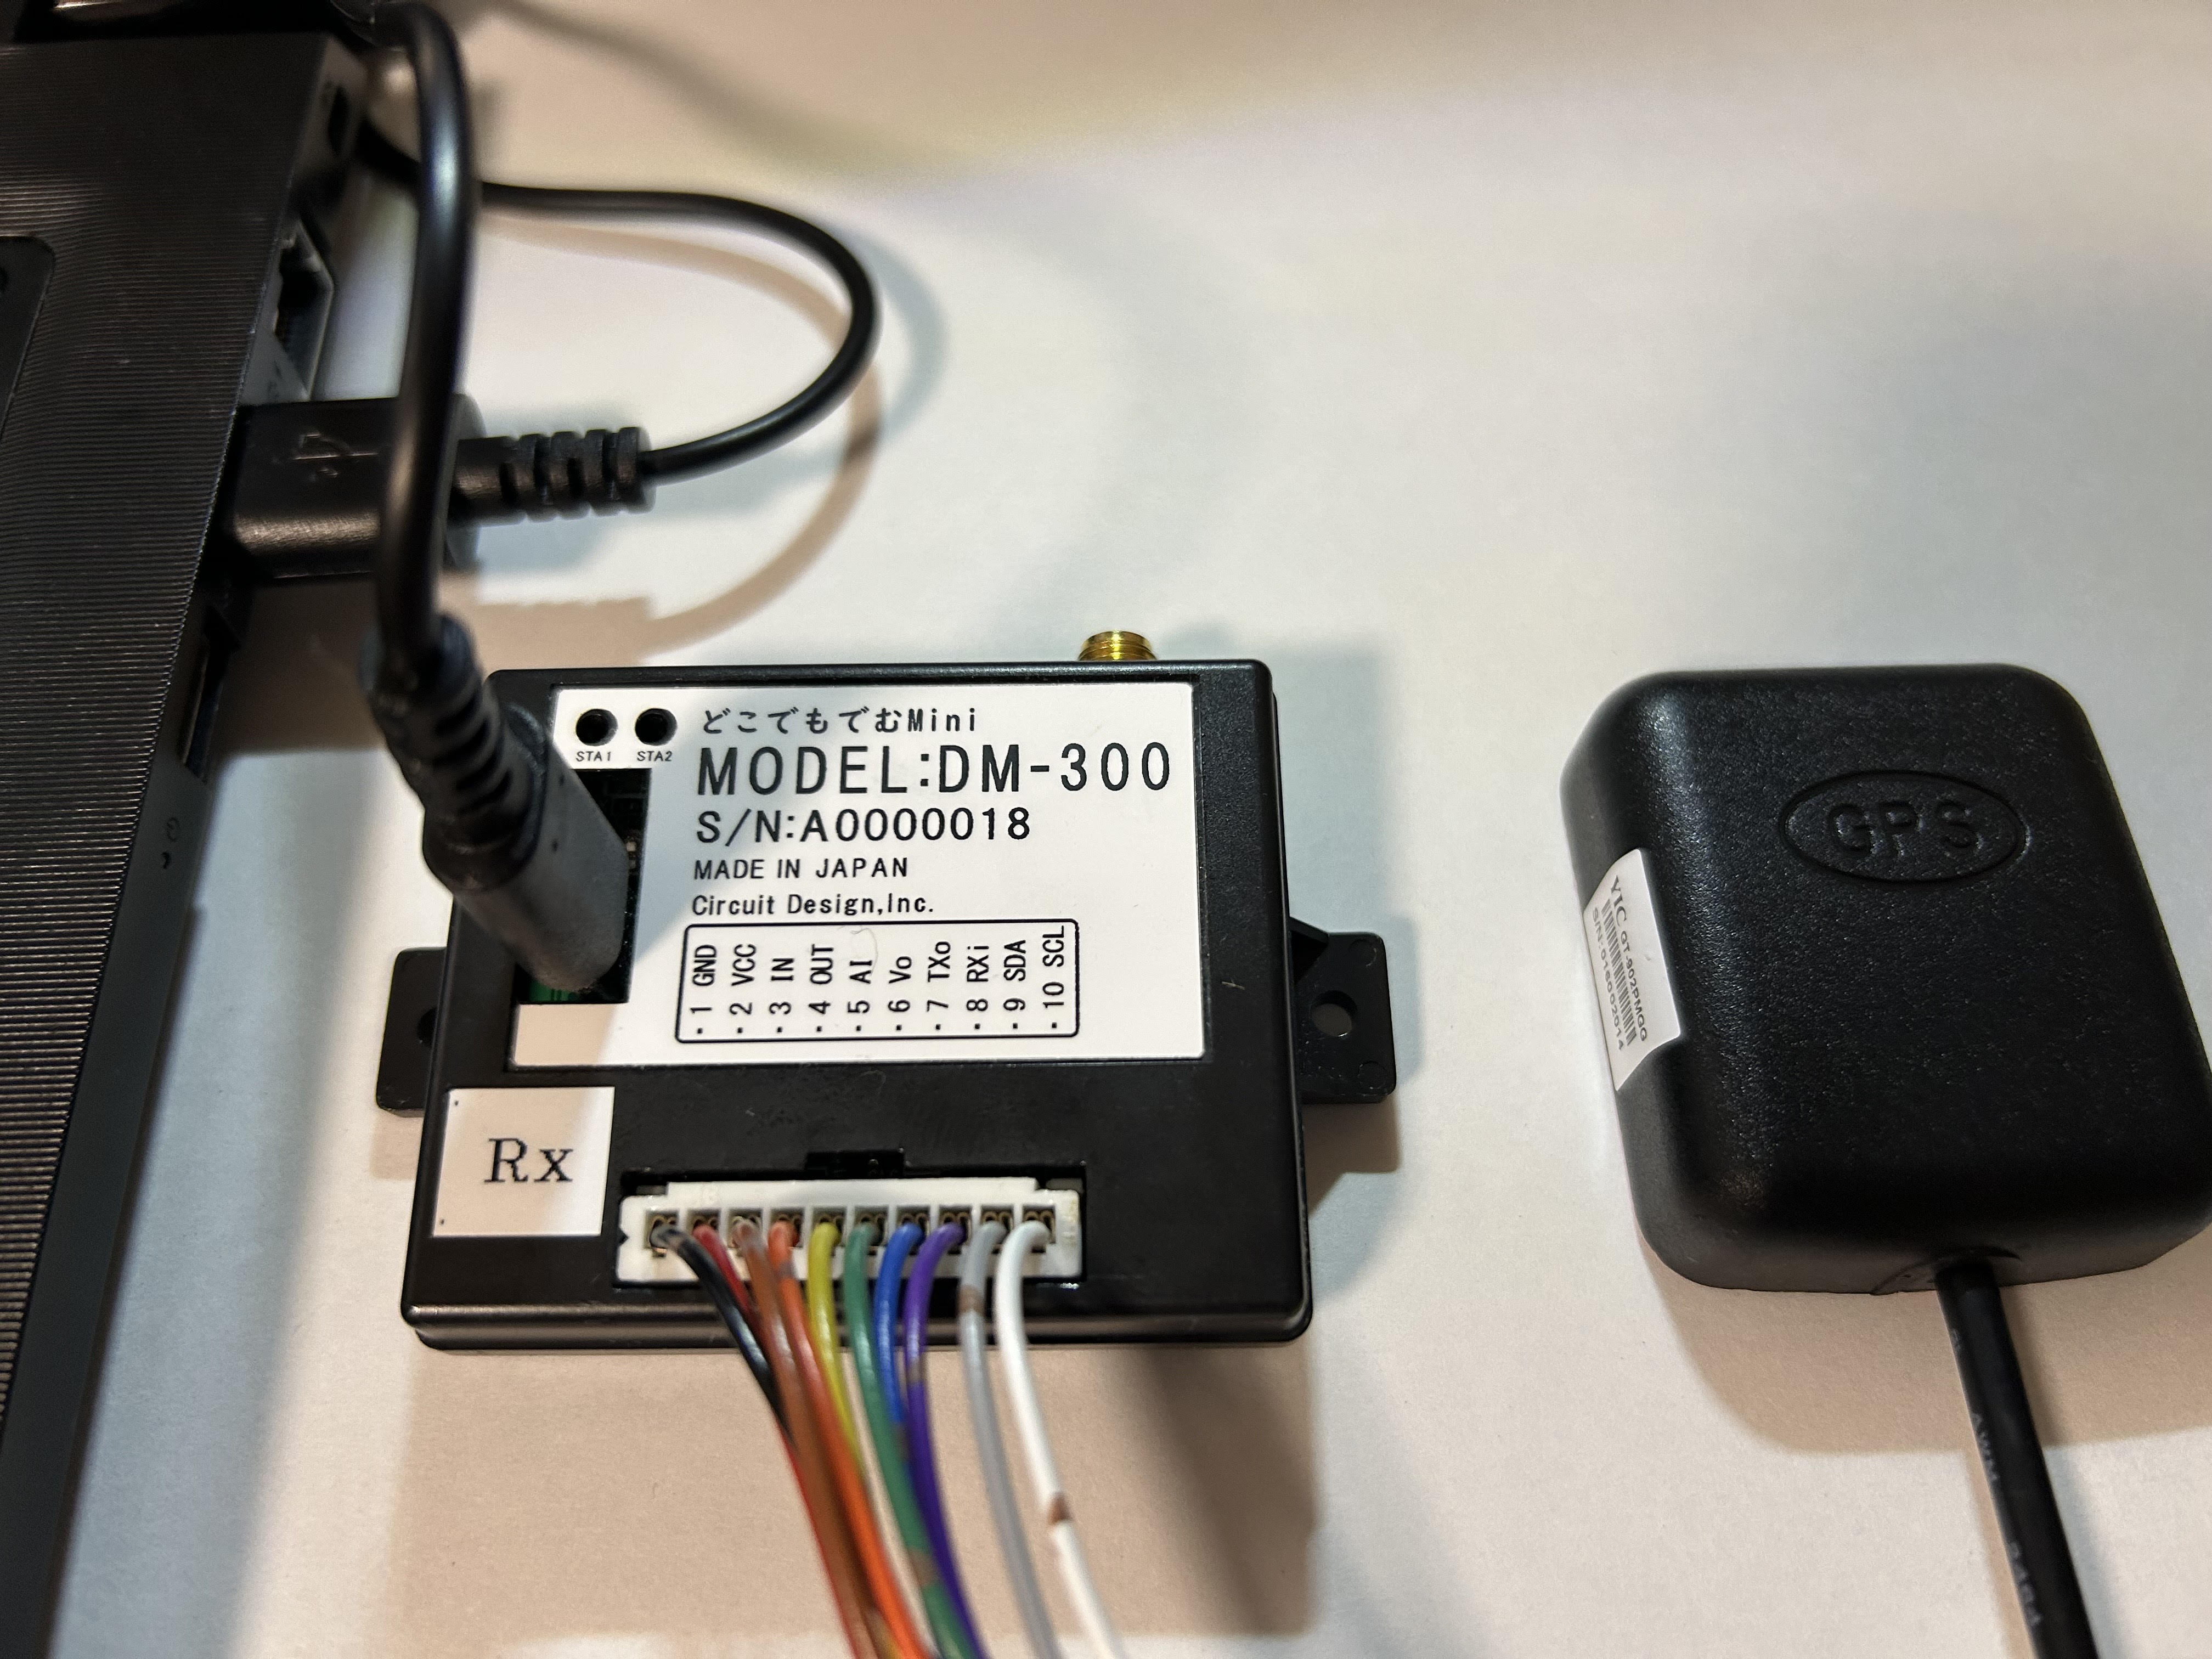
\includegraphics[width=60mm]{./images/devices.jpg}
  \caption{どこでモデム(左)とGPSモジュール(右)}
  \ecaption{Block diagram of the proposed system.}
  \label{fig:system}
\end{figure}

\subsection{デバッグシステム部}
本節では,通信プロトコルの動作を可視化し,逐次的なデバッグを可能とするデバッグシステムについて述べる。
提案システムは,通信処理中に出力されるログ情報を活用し,ブラウザ上で状態遷移の再現・変数追跡を行うことで,
開発者が通信の挙動を直感的に理解できる環境を提供する。
\vskip\baselineskip

\subsubsection{UI構成}
図4に本システムの可視化画面を示す。画面上部にはログファイルおよび状態遷移図ファイルのアップロード領域があり,
中央にはステップ実行ボタンとスライダーが配置されている。下部には,変数追跡領域・ログ表示領域・状態遷移図描画領域が横並びに配置されており,通信処理の進行状況を統合的に把握できる構成となっている。
\vskip\baselineskip

\subsubsection{ログ出力}
通信処理中の各状態遷移および変数の変化は,ファームウェア内で逐次的にログとして出力され,テキストファイルとして保存される。ログは識別タグを付与したシンプルな形式を採用しており,各行において状態または変数の情報を明確に区別できる。これにより,後述の可視化システムにおいて  状態遷移と変数変化を容易に解析できる。ログファイルの一例を以下に示す。
\vskip\baselineskip

\subsubsection{可視化・再現機構}
記録されたログファイルと,状態遷移図の構造を記述したJSONファイルをブラウザ上でアップロードすることで,Mermaid.jsを用いた状態遷移の可視化および再現を行う。Mermaid.jsはテキストベースで状態遷移図を描画できるJavaScriptライブラリであり,ログの進行に合わせて図中の状態ノードが順次ハイライトされる。これにより,通信処理の進行状況を視覚的に確認できる。状態遷移図のJSONファイルは,以下のような形式で各状態と遷移関係を定義している。
\vskip\baselineskip

\subsubsection{ステップ実行及び変数追跡}
可視化画面には,ログ再現を操作するための「次のステップ」「前のステップ」「最初に戻る」ボタン,および任意位置に移動可能なスライダーが実装されている。これにより,通信動作の経過を1ステップずつ追跡しながら確認することができる。また,特定の変数を選択してその値の変化を随時表示する機能を備えており,
状態遷移と変数変化の対応関係を同時に把握できる。これらの機能により,異常動作が発生した際の原因追跡を効率的に行える。
\vskip\baselineskip

\subsubsection{リアルタイム可視化}
さらに,本システムの拡張として,MQTTおよびSocket通信を利用したリアルタイム可視化機能の試作を行った。これにより,実機から送信されるログデータを逐次受信し,ブラウザ上で即時に状態遷移を反映することが可能となった。通信プロトコルのリアルタイム動作を視覚的に確認できる点で有用であるが,通信周期が短い場合は状態遷移が高速に変化するため,視認性に課題が残る。
\vskip\baselineskip


% UIの画像
\begin{figure}[tb]
  \centering
  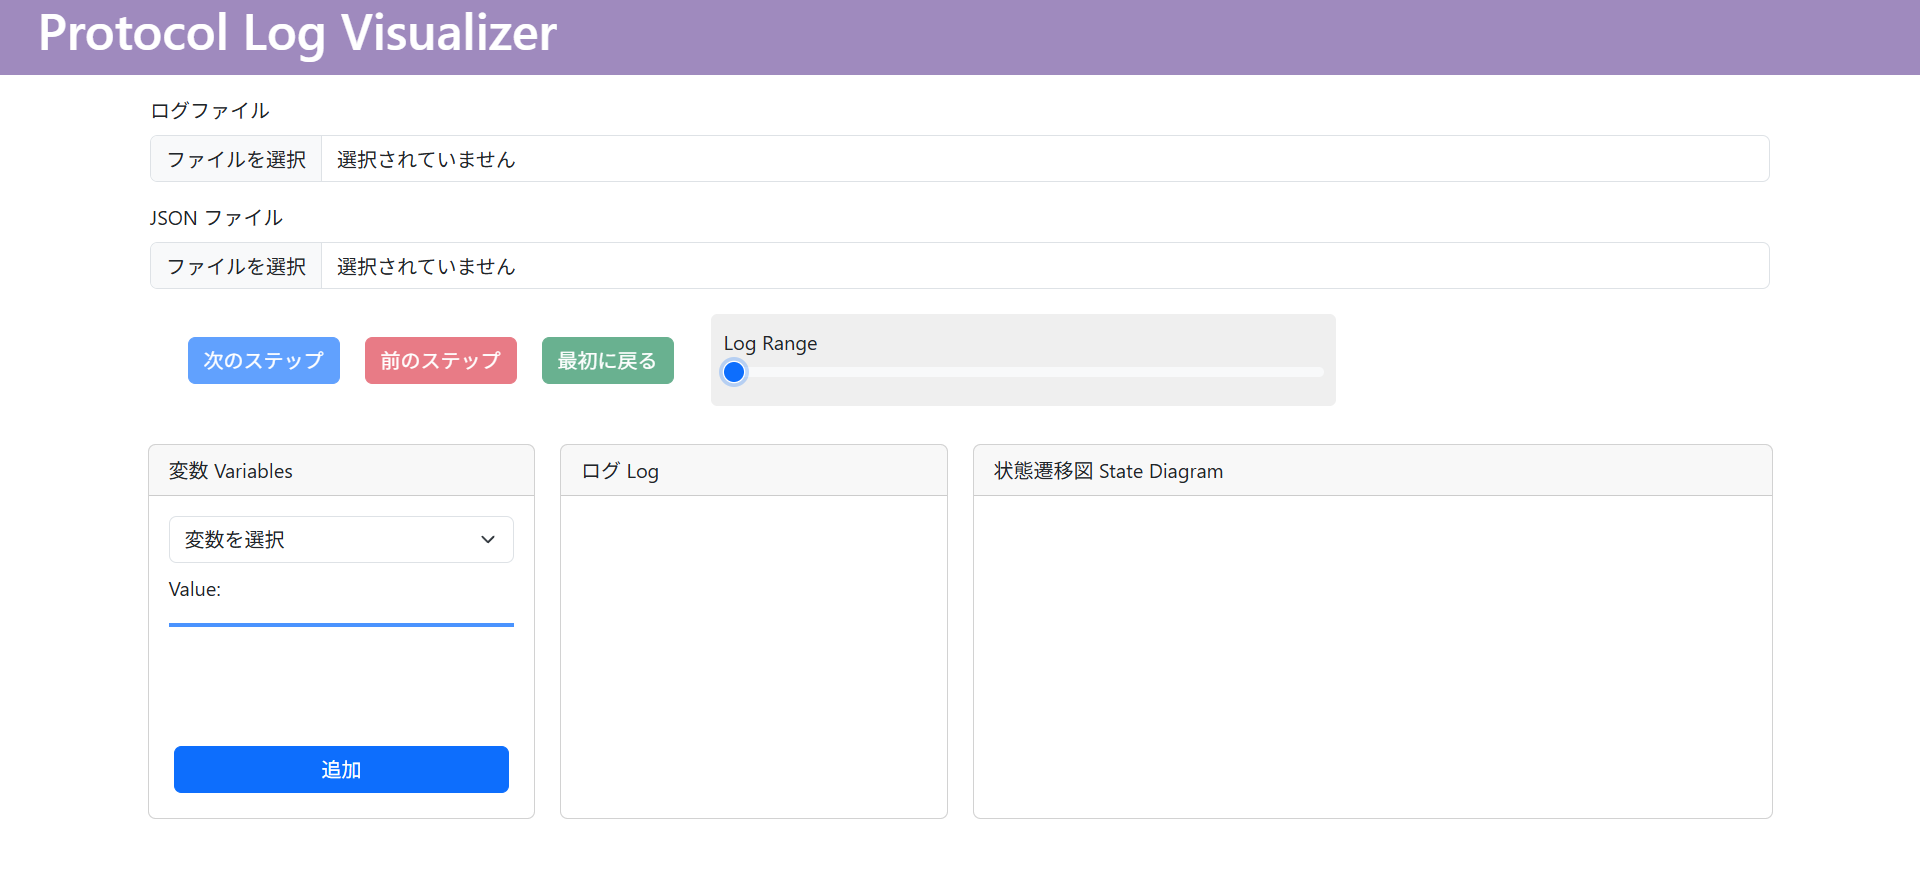
\includegraphics[width=80mm]{./images/viewer_ui.png}
  \caption{ログ可視化・ステップ実行環境のUI}
  \ecaption{User interface of the log visualization and step execution environment.}
  \label{fig:viewer-ui}
\end{figure}

  % ステップ実行の画像
  \begin{figure}[tb]
    \centering
    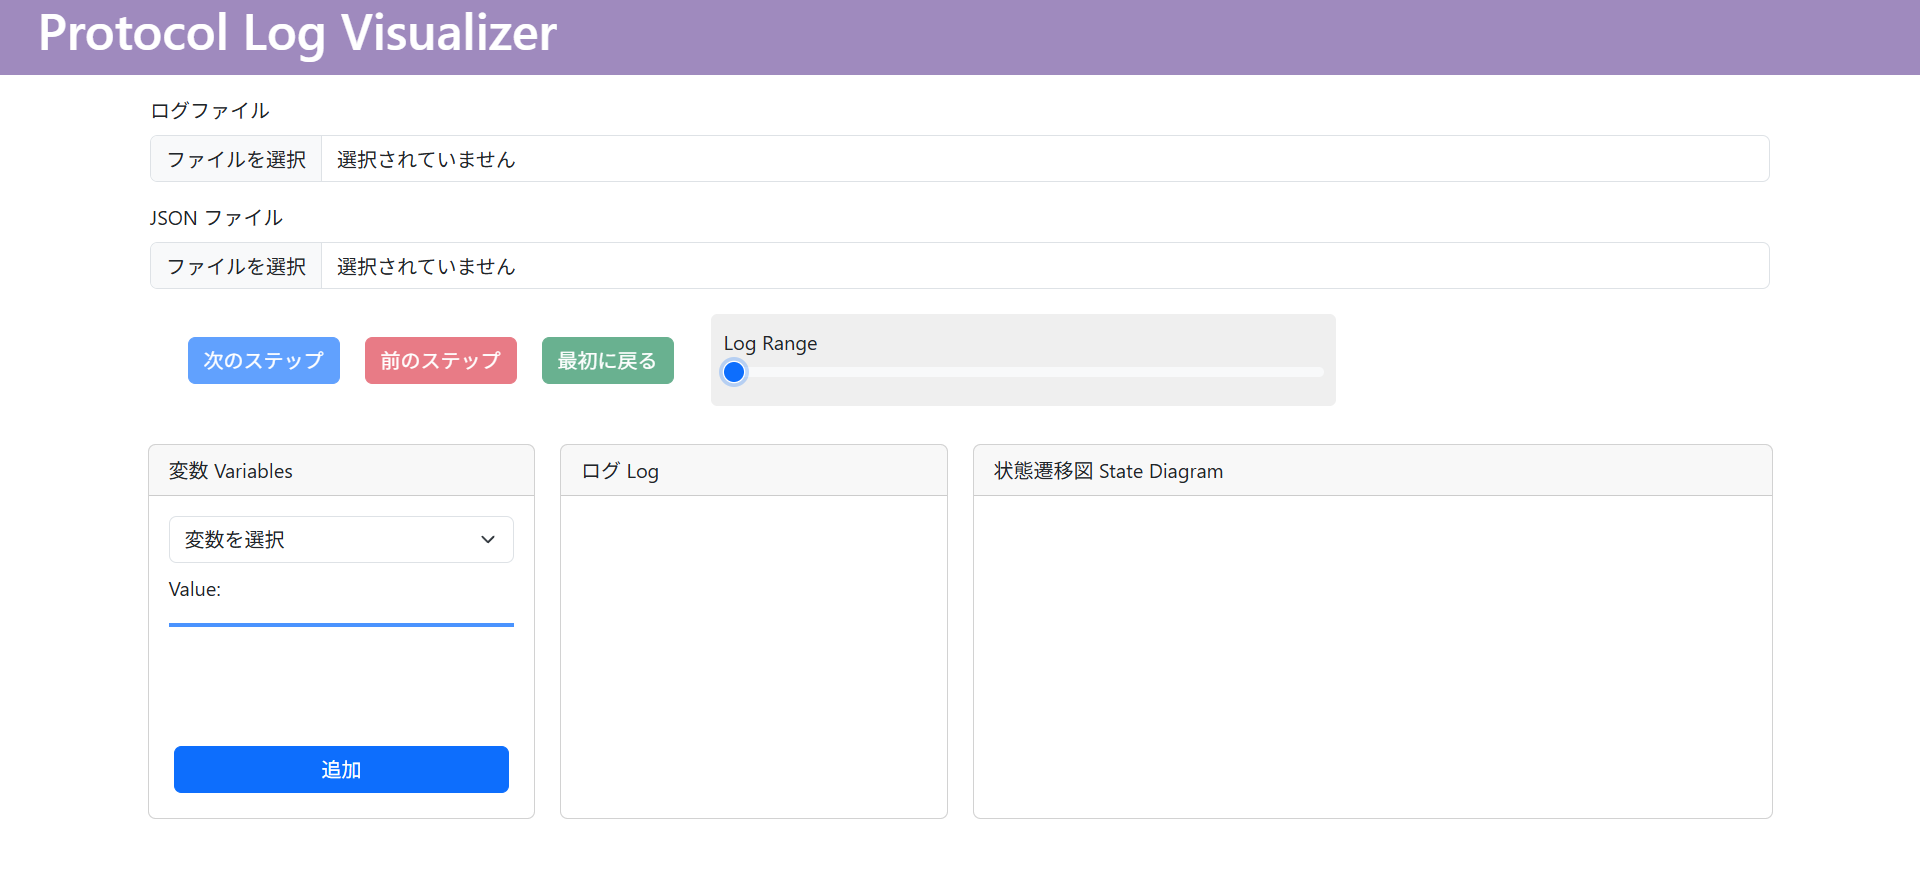
\includegraphics[width=80mm]{./images/viewer_ui.png}
    \caption{ログ可視化・ステップ実行環境のUI}
    \ecaption{User interface of the log visualization and step execution environment.}
    \label{fig:viewer-ui}
  \end{figure}


% _/_/_/_/_/_/_/_/_/_/_/_/_/_/_/_/_/_/_ 3章 /_/_/_/_/_/_/_/_/_/_/_/_/_/_/_/_/_/_/_/_/_/_/_/_/_/_/_/_/_/_/
\section{プロトコル実装と評価}

\subsection{プロトコルの実装}
状態遷移図をもとに自動生成されたファームウェアを実機に適用し、独自プロトコルを実装した内容を説明。
書くべき内容:
使用した状態遷移図の概要(図7)
各状態の役割(IDLE, TRANSMIT, WAIT\_ACK など)
コード生成後にPlatformIOで実行可能になるまでの流れ(図1〜図7とつなぐ)
どのようにスロット割当・送信・ACK処理を行うか(簡略な説明)
図7は簡略化している旨を明記(→論理構造に焦点)

例文イメージ:
状態遷移図から自動生成されたプログラムをどこでモデム上で実行し、信大独自プロトコルを実装した。図7に本プロトコルの主要な状態遷移を示す。本図は、実装上の例外処理や再送制御を省略し、主要な動作経路を示している。
% 開発したプロトコルの状態遷移図
\begin{figure}[b]
  \centering
  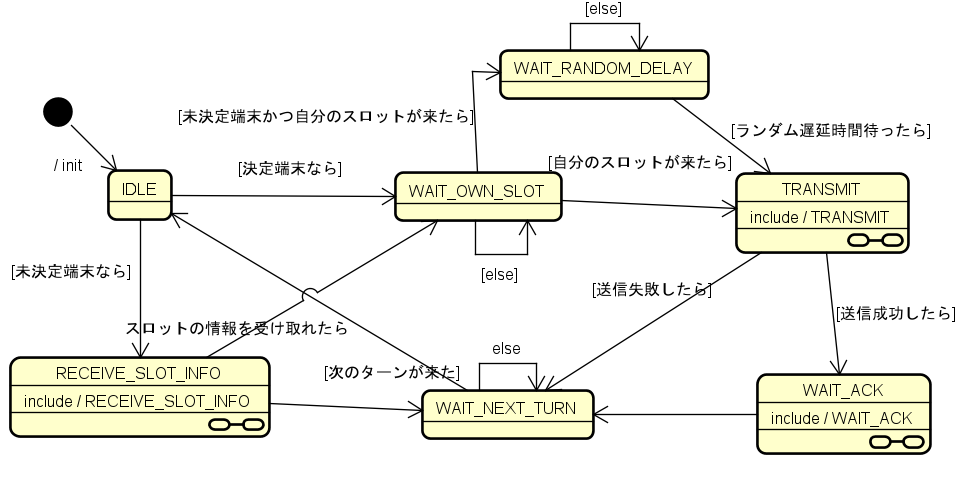
\includegraphics[width=80mm]{./images/protocol-state-machine3.png}
  \caption{開発した無線通信プロトコルの状態遷移図.
※実装上の詳細条件や内部処理は簡略化して記載している.}
  \ecaption{State transition diagram of the developed wireless communication protocol.}
  \label{fig:protocol-state-machine}
\end{figure}

\subsection{実験}
実際に複数ノードで通信を行い、ログを取得した環境と条件。

書くべき内容:

実験環境(図1の汎用ハードウェア構成を引用)

送受信ノードの台数・配置(例:2ノード間通信で検証)

検証項目:「通信状態の追跡」「デバッグの効率」「ログ可視化の有用性」

例文イメージ:

実験では,送信ノードと受信ノードの2台構成で通信プロトコルを動作させた。各ノードはSAMD21マイコンを搭載した無線モデム上で動作し,状態遷移ごとにログを出力した。これらのログをブラウザ上に読み込み,状態遷移図と変数を逐次可視化することで,プロトコルの動作確認および異常時の原因追跡を行った。

\subsection{評価}
「従来との比較」「有効性の実証」「教育的有用性」を軸に。

書くべき内容:

コンソール出力のみとの比較(表 or 図)

可視化ツール使用時の違い(例:デバッグ時間短縮・理解のしやすさ)

図8として「ログビューワ画面」を掲載(実際のUIキャプチャ)

ステップ実行中の状態変化を図9として掲載

例文イメージ:

図8に提案システムの可視化画面を示す。ログファイルをアップロードすると,通信プロトコルの状態遷移がブラウザ上で描画される。
図9にステップ実行中の画面を示す。現在の状態がハイライトされ,変数の値が逐次更新されることで,通信処理の挙動を直感的に把握できる。
従来はコンソールログを手動で追う必要があったが,本システムにより動作過程を一目で確認でき,デバッグ時間が大幅に短縮された。


本システムの有効性を確認するため,状態遷移図から自動生成したコードを用いて無線通信プロトコルを実装し,複数端末間での通信を行った。その際に出力されるログをブラウザに取り込み可視化することで,プロトコルの状態遷移を逐次的に追跡できることを確認した。

従来はコンソール出力のみに依存していたため,高速に進行する通信処理の挙動を逐一把握することは困難であった。本システムではログを視覚的に再現し,ステップ実行形式で確認できるため,デバッグ効率の向上に寄与することを示した。
% デバッグ方法の比較画像
% 従来の方法
\begin{figure}[tb]
  \centering
  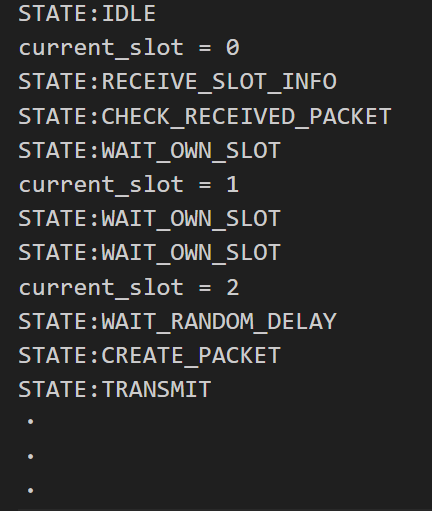
\includegraphics[width=50mm]{./images/old_debug.png}
  \caption{従来のコンソールによるデバッグ方法}
  \ecaption{Example of the old console-based debugging method.}
  \label{fig:old-debug}
\end{figure}
% 提案システム
\begin{figure}[tb]
  \centering
  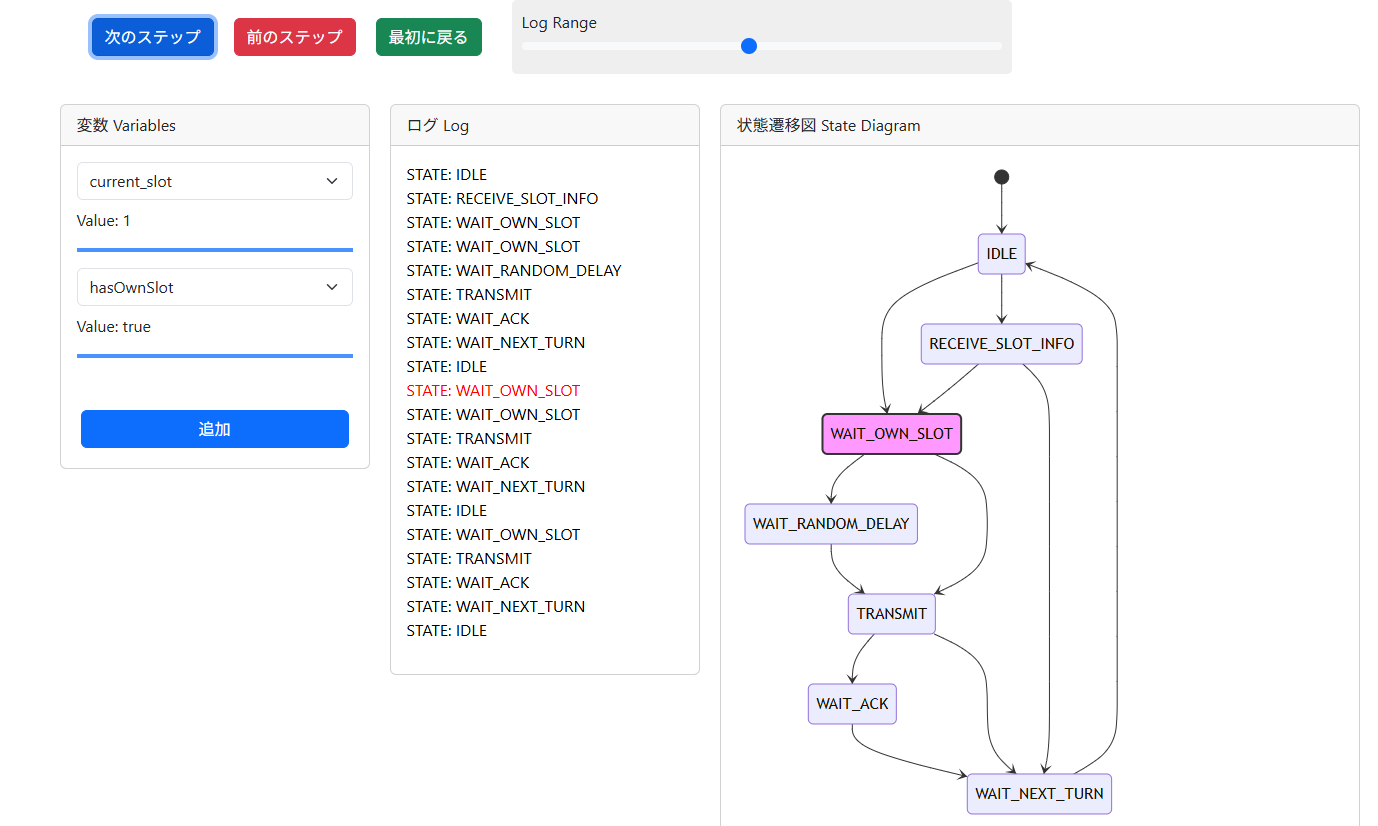
\includegraphics[width=80mm]{./images/step_3.png}
  \caption{提案システムによるログ可視化・ステップ実行環境}
  \ecaption{Log visualization and step execution environment of the proposed system.}
  \label{fig:viewer-ui}
\end{figure}


% _/_/_/_/_/_/_/_/_/_/_/_/_/_/_/_/_/_/_ 4章 /_/_/_/_/_/_/_/_/_/_/_/_/_/_/_/_/_/_/_/_/_/_/_/_/_/_/_/_/_/_/
\section{考察}
本研究で開発したログ可視化システムにより,通信プロトコルの動作過程を逐次的に追跡できることを確認した。これにより,従来のコンソール出力のみに依存したデバッグ手法に比べて,通信動作を直感的かつ体系的に理解することが可能となった。特に,状態遷移図上で現在の状態や変数の変化を視覚的に把握できる点は,デバッグ効率の向上に大きく寄与する。

従来手法では,高速で進行する通信処理の挙動を逐一確認することが困難であり,異常動作の再現や原因特定に多くの時間を要していた。本研究の可視化環境では,ステップ実行機能により状態遷移を一段階ずつ再現できるため,処理の流れや条件分岐を容易に追跡できる。これにより,開発者が異常箇所を迅速に特定できるだけでなく,通信アルゴリズムの学習や設計意図の共有にも有効である。

また,開発した環境は教育的利用や共同研究にも有用であると考えられる。例えば,状態遷移図を教材として利用する際に,図上で通信動作を再現できることは,通信プロトコルの理解促進に寄与する。さらに,複数の開発者がログを共有しながら解析を行うことで,チーム開発時のコミュニケーション効率の向上も期待できる。

一方で,現時点のシステムにはいくつかの課題が残る。第一に,リアルタイム性の向上が挙げられる。現状では,ログを取得後に可視化する「事後解析型」が中心であり,実機動作中の挙動をリアルタイムで完全に再現するには至っていない。第二に,通信性能やデバッグ効率の改善効果を定量的に評価していない点である。定量的な指標に基づく評価を行うことで,提案システムの有効性をより客観的に示すことができると考えられる。第三に,ノード数の増加に伴うログ量の増大や可視化負荷への対応も今後の検討課題である。

総じて,本研究の成果は,通信プロトコルの開発・理解・教育を支援する基盤として有効であることを示唆しており,さらなる拡張によって幅広い応用が期待される。

\vskip\baselineskip


% _/_/_/_/_/_/_/_/_/_/_/_/_/_/_/_/_/_/_ 5章 /_/_/_/_/_/_/_/_/_/_/_/_/_/_/_/_/_/_/_/_/_/_/_/_/_/_/_/_/_/_/
\section{まとめおよび今後の展望}
本研究では,状態遷移図から自動生成したファームウェアを汎用ハードウェア上で実行し,無線通信プロトコルの動作を実機で検証可能とする環境を開発した。さらに,通信処理中に出力されるログを解析し,ブラウザ上で状態遷移および変数変化を可視化・ステップ実行できるデバッグ支援システムを実装した。

これにより,従来のコンソール出力によるデバッグでは困難であった逐次的な動作確認を可能とし,プロトコル動作の理解促進と開発効率の向上に寄与することを示した。また,状態遷移図を中心とした設計と可視化環境の統合により,通信プロトコルの設計・実装・評価を一貫して行える開発基盤を実現した。

今後の展望としては,以下の3点を挙げる。
\begin{enumerate}
\item \textbf{定量的評価の実施:} デバッグ時間やエラー検出効率などを指標として,提案システムの有効性を客観的に評価する。
\item \textbf{大規模ネットワークへの拡張:} ノード数を増加させた環境での通信挙動の検証や可視化負荷の軽減手法の検討を行う。
\item \textbf{リアルタイム可視化機能の強化:} MQTTやSocket通信を活用したリアルタイムデータストリーム処理により,実時間での挙動確認を可能とする。
\end{enumerate}

また,社会的応用としては,登山者見守りシステムなどへの展開や,通信教育・実習環境への導入が有望である。さらに,将来的には,センサデータの可視化や異常検知アルゴリズムの統合など,応用層への拡張も視野に入れて研究を継続していく。


\vskip2\baselineskip
%\bibliographystyle{sieicej}
%\bibliography{myrefs}
\bibliographystyle{junsrt}
\begin{thebibliography}{99}
\bibitem{jst2022} 科学技術振興機構: 「SIP IoE 年次報告書 2022」, 2022.
\bibitem{mdpi2021} M. R. Hasan et al.: "Recent Advancement of Data-Driven Models in Wireless Sensor Networks," *Technologies*, vol.9, no.4, 2021.
\bibitem{asahi}
\bibitem{kobayashi2023} 小林遼, アサノデービッド, 不破泰:
“センサーネットワーク検証システムにおける遷移図を用いたMACプロトコル設計環境の開発,”
信学技報, NS2023-xx, 2023.

\bibitem{PlatformIO}
\bibitem{circuitdesign}
\bibitem{astah}
\bibitem{mermaid}
\end{thebibliography}
\end{document}


